% Appendix A
\label{AppendixA-methods} % For referencing this appendix elsewhere, use \ref{AppendixA}
\chapter{Methods} % Main appendix title

Procedures used to set up experiments are detailed in this appendix.

\section{Cleaning data}

Data corruption was found with Unity3D generated datasets where some .json files were not generated, leading to missing steering angles and throttle values for some images. There "orphaned" images were deleted with script src/utils/jsonclean.py

\section{Running the car simulator}
\label{RunningCarSimulatorForInference}

The main testing environment consisted of a Dell Precision Tower 5810 with a 6 core Intel Xeon Processor and 32GB memory running Ubuntu 18.04. Unity Hub 2.3.2 was installed then run as sudo:
\begin{verbatim}
$ sudo ./UnityHub.AppImage --no-sandbox 
\end{verbatim}
The car simulator source was cloned from:
\begin{verbatim}
$ git clone https://github.com/dsikar/sdsandbox.git    
\end{verbatim}
The Unity project contained in sdsandbox/sdsim can then added and loaded.
Once the menu scene runs, one of 5 circuits can be chosen. Once the chosen circuit is loaded, there are options to \textit{Auto Drive w Rec} (generate test data and steering angle using PID control) or \textit{NN Control over Network} (send images over network and receive predicted steering angles). The first case will output files to ../output directory, the second case will send and listen to network messages. The handshake process has been captured with tcpflow and stored to  src/debug/tcpflow\_output.txt. The prediction engine starts returning predicted steering angles after the 4th frame sent by simulator as described in section \ref{NetMonDebug}

\begin{figure}[ht]
 \centering 
 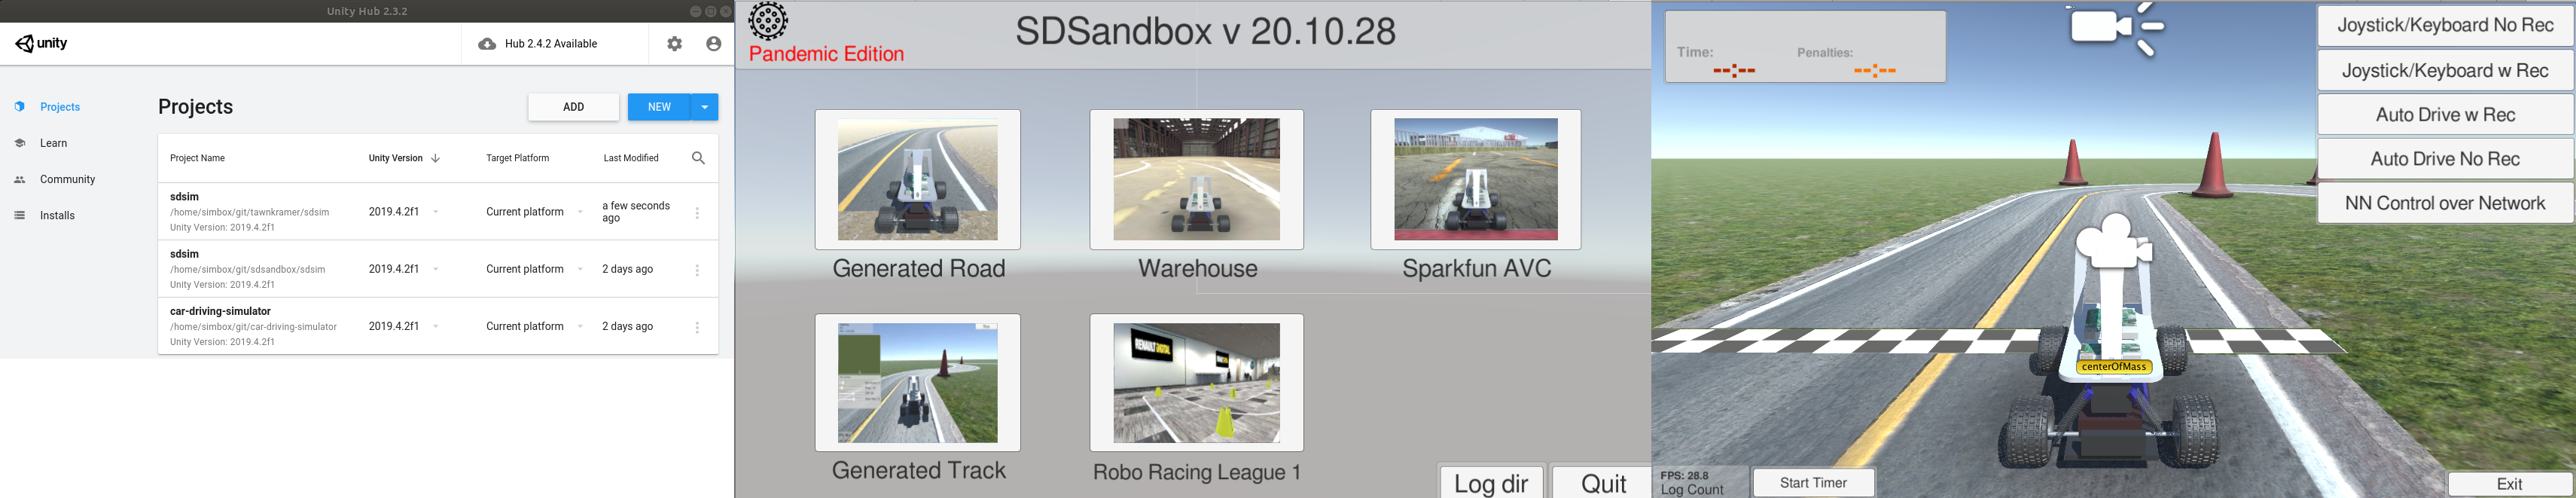
\includegraphics[scale=0.17]{Figures/UnityHubSDSandbox3in1.png}
 \caption{Left to right: Unity Hub, SDSandbox home screen and simulation ready to run}
 \label{fig:SDSandboxHome}
\end{figure}



\section{Network monitoring and debugging}
\label{NetMonDebug}
tcpflow (\cite{garfinkel2013passive}) was used to monitor network traffic between car simulator and neural network prediction engine. Once the simulator is setup to run in neural network mode and before the predict\_client.py prediction engine starts, tcpflow is launched set to listen on the loopback interface port 9091, and output network traffic packets to console:
\begin{verbatim}
$ sudo tcpflow -i lo -c port 9091
\end{verbatim}
The prediction script then runs, and JSON (\cite{pezoa2016foundations}) a lightweight data-interchange format, tcp packets may be monitored and debugged. Simulator packets are distinguished by \textit{telemetry} and prediction engine packets by \textit{control} msg\_types respectively, as shown in excerpt:
\begin{verbatim}
127. (...) {"msg_type":"telemetry",(...),"image":(...)
127. (...) {"msg_type": "control", "steering": "-0.09476048" (...)
\end{verbatim}
The packets carry the image sent from sim to prediction engine, and returned steering angle prediction.

\section{Generating Plots}

This section describe the tools used to generate plots.

\subsection{Steering angle comparison}

Plots were generated with Jupyter Notebook:
\begin{verbatim}
    src/utils/
\end{verbatim}

\section{Datasets}

A template directory structure was created such that downloaded data could be accessed in code with the same paths. The structure exists in the datasets repository and once cloned creates the template directory:
\begin{verbatim}
$ git clone https://github.com/dsikar/msc-data
$ tree -d msc-data/
msc-data/
 audi
 ford
 kitti
 mechanical-turk
 udacity
 unity
\end{verbatim}

\subsection{Ford AV Dataset}

The steering angles can be extracted from .bag files using ROS commands:
\begin{verbatim}
    # In one terminal, start ros engine
    $ roscore
    # In another terminal, inspect content of bag file
    $ time rosbag info Sample-Data.bag
    (...)
             /imu                 146939 msgs    : sensor_msgs/Imu             
    (...)
             /pose_ground_truth   146136 msgs    : geometry_msgs/PoseStamped   
             /pose_localized       16100 msgs    : geometry_msgs/PoseStamped   
             /pose_raw            146190 msgs    : geometry_msgs/PoseStamped   
(...)
    # And subscribe to topic of interest 
    $ rostopic echo /imu | tee sample_imu.yaml
    # In another terminal, playback bag file
    $ time rosbag play --immediate Sample-Data.bag --topics /imu
    # Sanity check, count number of acquisitions
    $ cat sample_imu.yaml | grep "orientation:" | wc -l
\end{verbatim}
The snippet above generates file imu.yaml, with all pose data generated by imu device. From this file we extract the steering angle, which is the z axis (yaw) of the orientation field (TODO check .yaml dialect). 
Images can be extracted from the same bag file with the Python 2.7 bag\_to\_images.py script:
\begin{verbatim}
    $ python2 bag_to_images.py Sample-Data.bag ~/git/msc-data/ford/sample/ros/ \
        /image_front_left
\end{verbatim}
Each image is an attribute in a dictionary, which also contains seconds (secs) and nano seconds (nsecs) attributes within the header attribute:
\begin{verbatim}
header: 
  seq: 213414
  stamp: 
    secs: 1501822147
    nsecs: 684951066
  frame_id: "camera_front_left"
height: 215
width: 414
encoding: "8UC3"
is_bigendian: 0
(...)
\end{verbatim}
Thus a timestamp can be obtained for each image extracted. This is done with script parse\_yaml\_time.py:
\begin{verbatim}
    
\end{verbatim}
While the steering angles are extracted 
The image can be matched with a steering angle by obtaining the timestamp of image, the full secs 

\section{Automold}
The rainy images were created with:  
\begin{verbatim}
github.com/dsikar/automold/RainyImagesDissertationPlot.ipynb
\end{verbatim}

\section{Development Environments}

\subsection{Intel DevCloud}

Intel provides a 200GB storage quota. Storage use can be checked with getquota command:
\begin{verbatim}
$ getquota
199.78 GB out of 200.00 GB (99.89%) used   
\end{verbatim}
Jobs are queued with qsub command:
\begin{verbatim}
    $ qsub -l nodes=1:gpu:ppn=2 ford_sample_download.sh -l walltime=23:59:59
\end{verbatim}
where the actual commands that run e.g. downloading data, training and testing networks are scripted in a batch file e.g. ford\_sample\_download.sh, train.sh.   
The queue can be checked with watch command:
\begin{verbatim}
    $ watch -n 1 qstat
\end{verbatim}
Jobs can run for a maximum of 24 hours, any job exceeding that execution time is terminated automatically. Jobs can be deleted from queue with qdel command.

\section{Unity}
Unity for Ubuntu is a single image file, that can be downloaded and run:
\begin{verbatim}
$ ./UnityHub.AppImage    
\end{verbatim}
This will start the Unity Hub app. A license must be installed by downloading a file, logging into Unity, uploading file then downloading a second license file. This is added to Unity Hub. The next step is to get an editor. Editors are available at:
\begin{verbatim}
https://unity3d.com/get-unity/download/archive    
\end{verbatim}
From archive pages, a link is obtained for desired editor (2019.3.0 is this case).
To load the editor, Unity Hub must be closed and the re-opened with the obtained link:
\begin{verbatim}
$ ./UnityHub.AppImage unityhub://2019.3.0f6/27ab2135bccf
\end{verbatim}
Source code for the simulator can then be cloned locally
\begin{verbatim}
git clone https://github.com/tawnkramer/sdsandbox.git    
\end{verbatim}
The project can then be added to Unity Hub by ADDing and navigating to sdsandbox/sdsim directory. It will then be listed on Unity Hub. Thereafter, Unity Hub can be started with
\begin{verbatim}
$ ./UnityHub.AppImage    
\end{verbatim}

\section{Tensorflow and Keras}
\label{methods:tensorflow-keras}
The versions used were 2.2.0 and 2.4.3 respectively. To ensure the same versions are installed in all development platforms, run:
\begin{verbatim}
$ pip install keras --user
$ pip install tensorflow --user
# to check versions
$ python3
>>> import keras
>>> keras.__version__
'2.4.3'
>>> import tensorflow
>>> tensorflow.__version__
'2.2.0'
\end{verbatim}
If the modules are already present in the environment, but a lower (earlier) version e.g.:
\begin{verbatim}
>>> tensorflow.__version__
'1.15.4'    
\end{verbatim}
it can be upgraded by running:
\begin{verbatim}
$ pip install --ignore-installed --upgrade tensorflow==2.2.0 --user
\end{verbatim}

\subsection{Recording one loop around a track}

To record the images and steering angles generated by going around a track once, on the terminal:
\begin{verbatim}
$ sudo ./UnityAppimage --no-sandbox
\end{verbatim}
Open the project in sdsim directory (commit ed0cc0b)

\subsection{Running simulator predictions}
\label{running-simulator-predictions}

To run predictions, and to monitor TCP traffic:
\begin{verbatim}
# Run unity from one terminal run:
$ sudo ./Unity.AppImage --no-sandbox
# To monitor TCP traffic, from another terminal run:
$ sudo tcpflow -i lo -c port 9091 > /tmp/tcpflow.log
# To run predictions, from another terminal run:
$ python predict_client.py \
--model=../trained_models/nvidia_baseline/20201120124421\_nvidia\_baseline.h5
\end{verbatim}

% there probably will not be enough time to use ROS at scale so parking this for now in appendix, might leave for future reference or remove
\section{ROS}
The Robot Operating System (\cite{quigley2009ros}) is middleware, that is, placed between the operating system an the application program. It helps manage complexity and distributed systems, such as a managing the process of recording several sensor outputs in a moving vehicle. The term "plumbing" is sometimes used, as parts of a distributed application are connection with "data pipes".  
ROS was used to store data from the FORD AV dataset.

% \section{Extracting steering angles with ROS}
Info on how to get a steering angle (YAW) using quaternions and the IMU data.

\section{Correspondence with supervisor}
\label{corr_with_super}
\subsection{Correspondence with Artur Garcez 1}
\begin{verbatim}
Garcez, Artur
Fri 14/02/2020 09:59
Hi Daniel,
See if you can find a data set which would offer you a systematic way of evaluating
how CNNs can be fooled by visual illusions caused by rain drops on the windscreen.
Artur
________________________________________
From: PG-Sikar, Daniel <Daniel.Sikar@city.ac.uk>
Sent: 14 February 2020 08:56
To: Garcez, Artur
Subject: MSC Data Science - Final year project

Hi Artur,

I am currently shopping around for a project. I have spoken to a couple of companies
but not sure data will be available in good time - ML applied to signal processing.

So I ask if you have any projects, ideally related to some kind of signal processing,
alternatively, anything related to computer vision which could potentially provide a
good hook for the self-driving car project we spoke (briefly) about?

Kind regards

Daniel - PT2    
\end{verbatim}

\section{Correspondence with authors}
\label{corr_with_authors}

\subsection{Correspondence with Urs Muller 1}
\label{urs_muller1}
Correspondence with \textbf{Urs Muller}, co-author of \cite{bojarski2016end}, with respect to network training settings.

\begin{verbatim}
From: Urs Muller <umuller@nvidia.com>Sent: 16 November 2020 19:30
To: PG-Sikar, Daniel <Daniel.Sikar@city.ac.uk>
Subject: Re: End to End Learning for Self-Driving Cars - Network Training Parameters

CAUTION: This email originated from outside of the organisation. 
Do not click links or open attachments unless you recognise the
sender and believe the content to be safe.

Hi Daniel,

We used the following settings (we haven't documented them in any publication):

loss function: MSE
optimizer: adadelta
learning rate: 1e-4 (but not really used in adadelta)
dropout: 0.25

Best regards,
Urs

From: PG-Sikar, Daniel <Daniel.Sikar@city.ac.uk>
Sent: Sunday, November 15, 2020 6:53To: Urs Muller <umuller@nvidia.com>
Subject: End to End Learning for Self-Driving Cars - Network Training Parameters
 
External email: Use caution opening links or attachments

Hi,

With respect to your network training, I am investigating the effect of noise 
(rainy images) on network performance, using your architecture as a baseline.

Would you be able to point me towards any documentation detailing loss function, 
learning rate, optimizer and layer droupout probabilities used when training 
your network?

Thanks in advance for any help and kind regards,

Daniel Sikar | MSc Data Science Candidate
School of Mathematics, Computer Science and Engineering
City University of London    
\end{verbatim}

\subsection{Correspondence with Urs Muller 2}
\label{urs_muller2}
\begin{verbatim}
Urs Muller <umuller@nvidia.com>
Tue 17/11/2020 11:47
CAUTION: This email originated from outside of the organisation. Do not click links or open attachments unless you recognise the sender and believe the content to be safe.

Hi Daniel,

Yes, correct. We cropped everything above the horizon. The lower edge of the crop is as low as possible before the road gets blocked by the hood of the car.

Best regards,
Urs
From: PG-Sikar, Daniel <Daniel.Sikar@city.ac.uk>
Sent: Tuesday, November 17, 2020 2:56
To: Urs Muller <umuller@nvidia.com>
Subject: Re: End to End Learning for Self-Driving Cars - Network Training Parameters
 
External email: Use caution opening links or attachments
Hi Urs,

Thanks for your reply. One more question with respect to the image size presented to your network - 66 pixel height by 200 width. Was this cropped from the size your camera sensors were generating? To keep only the road in the frame and omit anything above the horizon?

Kind regards,

Daniel    
\end{verbatim}

\subsection{Correspondence with Ankit Vora}
\label{ankit_vora}
Correspondence with \textbf{Ankit Vora}, co-author of \cite{agarwal2020ford}, with respect to extracting steering angles from rosbag files.

\begin{verbatim}
Vora, Ankit (A.) <avora3@ford.com>
Thu 05/11/2020 13:55
CAUTION: This email originated from outside of the organisation. 
Do not click links or open attachments unless you recognise the
sender and believe the content to be safe.

Hi Daniel,

The information you are looking for will be in the /pose_ground_truth message. 
That message represents the position and orientation of the vehicle.
You will have to convert quaternions to yaw, pitch, roll angles and
then use the yaw values.

Ankit
From: PG-Sikar, Daniel <Daniel.Sikar@city.ac.uk>
Sent: Wednesday, October 28, 2020 7:00 PM
To: Vora, Ankit (A.) <avora3@ford.com>
Subject: Ford AV Dataset - obtaining steering angles
 
Hi,
I am studying your AV datast and have extracted the /imu data from provided .bag files, 
I am trying to work out if the steering angle can be inferred from the data?
Your article states the dataset provides 6DOF pose estimation.
The extracted /imu topic looks like:

header:
  seq: 137596
  stamp:
    secs: 1501822140
    nsecs: 610330104
  frame_id: "imu"
orientation:
  x: 0.00133041249526
  y: 0.00486443211508
  z: 0.584795486661
  w: 0.811165091756
orientation_covariance: [0.0, 0.0, 0.0, 0.0, 0.0, 0.0, 0.0, 0.0, 0.0]
angular_velocity:
  x: -0.0018081133007
  y: -0.0105949952451
  z: -0.00118502619208
angular_velocity_covariance: [0.0, 0.0, 0.0, 0.0, 0.0, 0.0, 0.0, 0.0, 0.0]
linear_acceleration:
  x: -0.0136899789795
  y: 0.199539378285
  z: 0.305044800043
linear_acceleration_covariance: [0.0, 0.0, 0.0, 0.0, 0.0, 0.0, 0.0, 0.0, 0.0]

I guess I am interested in the yaw, which would be the value z, but
having looking at the pattern it does not look like an angle that
could be associated to steering, positive and negative values close
to zero.

Could you help me identify the steering angle, or if it is not
present suggest any approaches to extract it from the data?

Anyway help would be greatly appreciated.

Daniel Sikar
Daniel Sikar | MSc Data Science Candidate
School of Mathematics, Computer Science and Engineering
City University of London   
\end{verbatim}

\subsection{Correspondence with Maxime Ellerbach}
\label{corr:ellerbach}
On the majority of the Donkey Race community using behavioural cloning for self-driving CNN training.

Maxime Ellerbach is the main maintainer of the SDSandbox project. 

\begin{verbatim}
Maxime Ellerbach
	
14 Nov 2020, 14:44 (4 days ago)
	
Oh, I think the drive menu is quite old, it was added before May update,
at this time Tawn was still doing the changes.
Now I'm the main maintainer of the project, for the moment I'm mainly
doing some backend changes to make the track creation process easier.

For the training part, most of us use behavioral cloning !
But they are mostly using the donkeycar framework, on my side I don't
use any framework and it performs great.
I would be happy if you could join us in a next virtual race !

Cheers,
Maxime

-----Message d'origine-----
De : Daniel Sikar <dsikar@gmail.com>
Envoyé : samedi 14 novembre 2020 15:25

À : Maxime Ellerbach <maxime@ellerbach.net>
Objet : Re: SDSandbox output image size

Thanks, that is super helpful. What really helped me was the drive menu being added to
the Generated Track.
I have not checked closely the commit history (I have been following SDSandbox since
February) but given you have been the most active user I take it was from you.
I did add some data augmentation to training that I thought might be helpful for others
doing behavioural cloning, but understand that most (or all) of you in the virtual race
league are using reinforcement learning models, making more use out of the Dokey-Gym
environment than I am. Anyway, I hope to get to RL before long and to join the league!
Daniel

\end{verbatim}

%%%%%%%%%%%%%%%%%%%%%%%%%%%%%%%%%%%%%%%%%%%%%%%%%%%%%%%%%%%%%%%%%%%%%%%%%%%%%
% Mechanical Turk
%%%%%%%%%%%%%%%%%%%%%%%%%%%%%%%%%%%%%%%%%%%%%%%%%%%%%%%%%%%%%%%%%%%%%%%%%%%%%

\section{Locating rainy sections with Mechanical Turk}
For Mechanical Turk, the data that looked most promising was Ford V2 Log 1 and V3 Log 1, both described as "freeway, overpass, bridge, cloudy". We drew 50 images uniformly from each log and added 5 images with rain that were expected to be labelled as such. The 105 images were then added to a SageMaker Ground Truth job. The platform works as a wrapper around Mechanical Turk as it facilitates the creation of user interfaces (Figure \ref{fig:MechTurkCreateJob})
% rainy files created with automold/RainyImagesDissertationPlot.ipynb
\begin{figure}[h!]
\centering
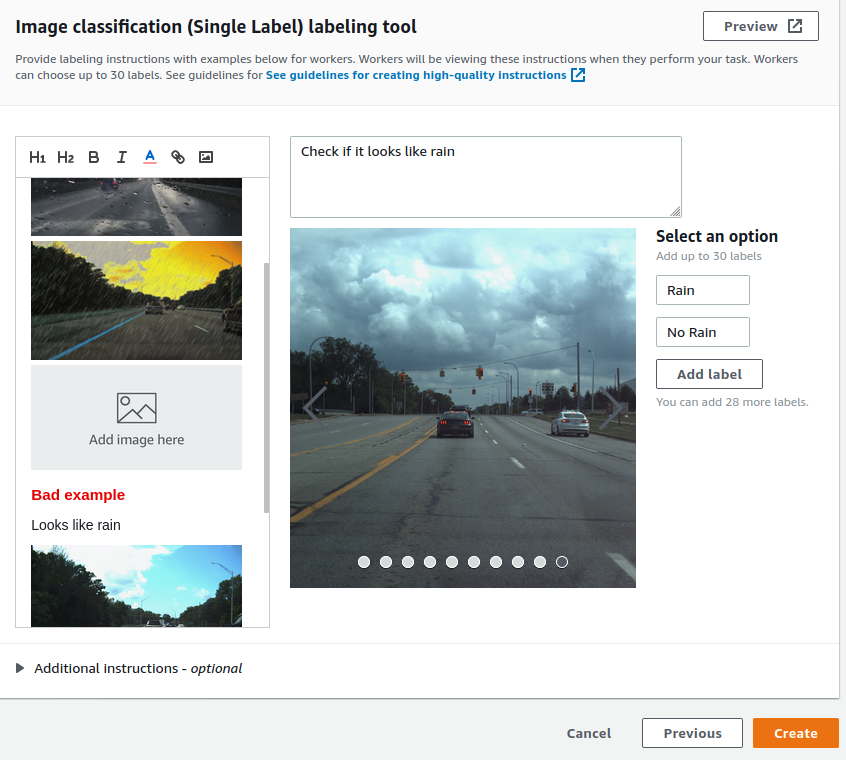
\includegraphics[width=10cm]{Figures/MechTurkCreateJob.png}
\caption{The SageMaker Ground Truth user interface template with two labels ("Rain", "No Rain"), the image to be labeled and examples of correct and incorrect classifications.}
\label{fig:MechTurkCreateJob}
\end{figure}
Labeling tasks are classified as low, medium and high complexity. The prices range from \$0.012 for a low complexity task, with a 5 second estimate to complete, to \$1.20 for a high complexity task with a 3.5 minute estimate to complete.
The task can be configured with an output for time taken by a worker on a single task, the lowest time interval being one minute.
There is also an option to assign more than one worker per dataset object, on account that it can help increase the accuracy of the data labels.
The task was created with the most basic options of one worker, a \$0.012 price per task, a one minute timeout and remained live for 12 hours. 
The images were labelled by Mechanical Turk workers and results made available in a json encoded file (datasets/mechanical-turk/2020-11-21\_22 45 37.json) showing no images had been labeled as "Rain". The assumption then being there are no sections containing rain in the dataset. The Automold library added rain images were also labeled as "No Rain". Figure \ref{fig:MechTurkLabeledImages}
\begin{figure}[h!]
\centering
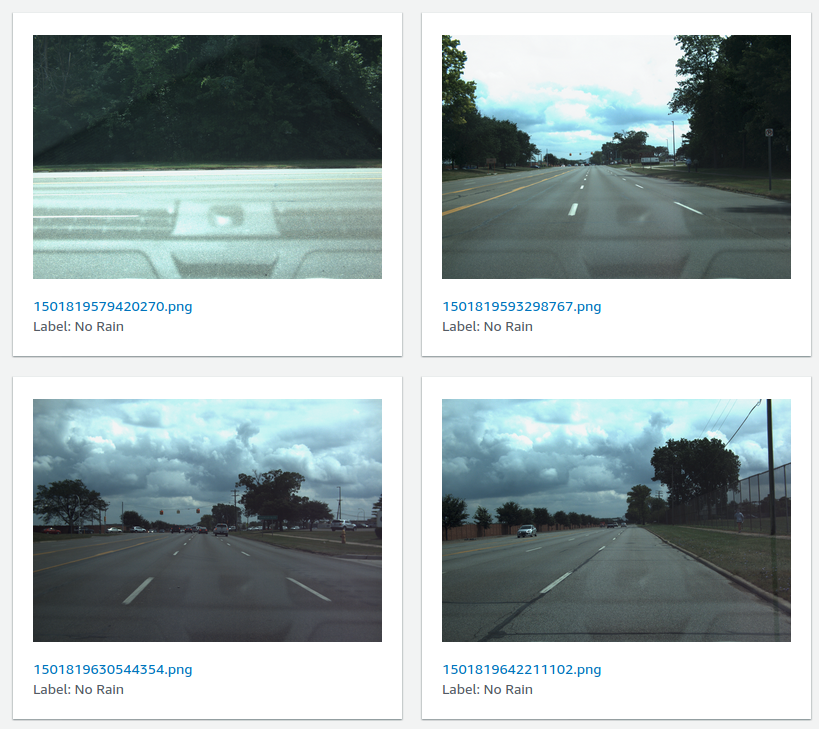
\includegraphics[width=10cm]{Figures/MechTurkLabeledImages.png}
\caption{The SageMaker Ground Truth labeled images detail on Labeling Job Summary page}
\label{fig:MechTurkLabeledImages}
\end{figure}